%
\section{Field line Integration}\label{cap:fieldlineintg}
%
This section refers to the \texttt{subroutine fieldline\_integrals} in TIEGCM. \\
%

The electrodynamo equation is reduced to two dimensions
assuming that the field--lines
are equipotential due to the high conductivity along the field--line.
The variable along the field line is $s$, and ${s_L}$ and ${s_U}$ are
the lower and upper boundary
of the line--integration. The inclination of the geomagnetic field--line at the
reference height $h_0$ on an assumed spherical Earth is $I_m$, and $B_{e3}$ is 
the component of the geomagnetic field along the field--line. Note that all value,s except
the geopotential height $z$, are stored on half pressure levels to make the integration more
convenient. \\
%
\begin{figure}
  \centering
  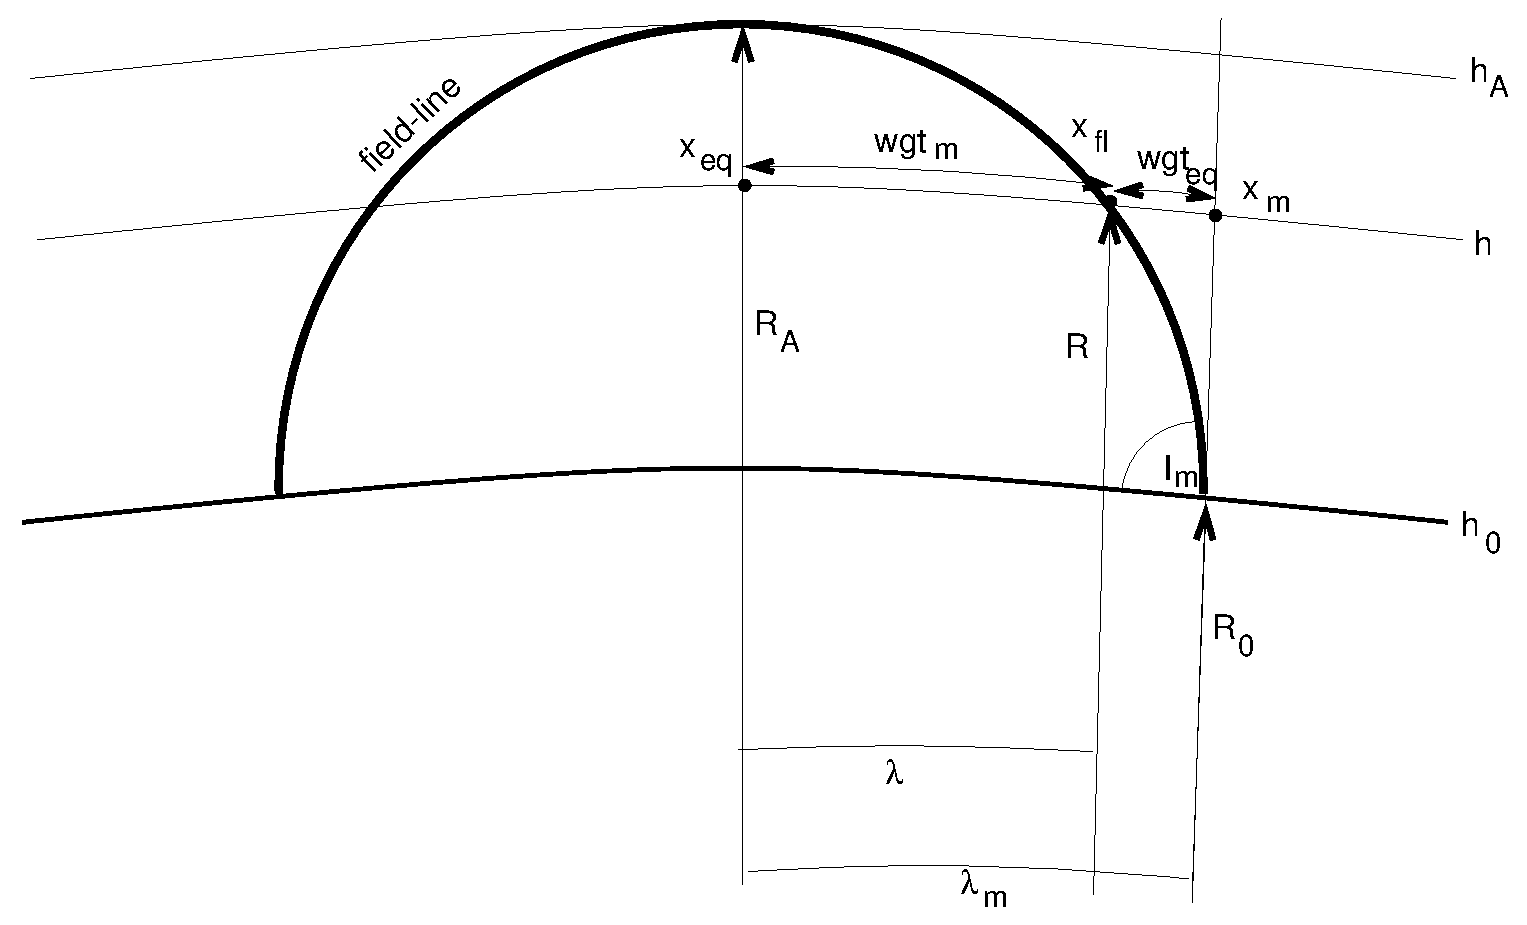
\includegraphics[scale=0.3]{./tex_plot/fl_geometry.eps}
  \caption{Sketch of geometry for the field--line integration}
   \label{fig:fieldline_intg}
\end{figure}
%
\paragraph{Approximation of field line values}
%
The correct way to do the field line integration would be to trace points along
the field line. However, the geomagnetic grid in TIEGCM is not oriented along the field line,
and therefore the tracking
would involve a two dimensional search and an interpolation to calculate the value on the field
line. This can be computational expensive and therefore an approximation, which should be close
to the true field line integration, is used.
The field line integration is approximated by a height integration 
combined with an interpolation
between the height-varying values at the foot point of the field line ($\lambda_m$, h) and the magnetic 
equator ($\lambda_m = 0, h$) (see. figure  \ref{fig:fieldline_intg}). Hence, only the height varying values at the foot point location 
$(\lambda_m, h)$ are needed.
Figure \ref{fig:fieldline_intg} shows schematically
a field line with the foot point latitude $\lambda_m$ at the reference height $h_0$. The
value $x_{fl}$ at height $h$ on the field line is approximated by the 
value $x_{eq}$ at the equator and height h
and the value $x_m$ at foot point latitude $\lambda_m$ and height h.
%
\begin{equation}
 x_{fl} = wgt_{eq} x_{eq} + wgt_m x_m \label{eq:approx_fl}
\end{equation}
%
with the weights $wgt_{eq}$ for the equator value and $wgt_{m}$  for the foot point value. 
From figure \ref{fig:fieldline_intg} the weight can be found as
%
\begin{equation}
 wgt_{eq} = \frac{\lambda_m -\lambda}{\lambda_m} \approx  
            \frac{sin(\lambda_m -\lambda)}{\lambda_m} \label{eq:wgh1}
\end{equation}
%
assuming that the difference $\lambda_m -\lambda$ is small, which is true close to the
foot point of the field line. Note that determining $\lambda$ would involve searching for the
point on the field line at height h which is time consuming, thus the sinus is used.
For field lines which foot point is at mid-- and height latitude the value on the
field line is essentially the height--varying value at the foot point, since the field line is
almost vertical.
Close to the magnetic equator the approximation is not so good anymore but the inaccuracy 
can be neglected when compared to the total field line integration.
 The term
$sin(\lambda_m -\lambda)$ can be substituted by
%
\begin{equation}
 sin(\lambda_m -\lambda) = sin \lambda_m cos \lambda - cos \lambda_m sin \lambda \label{eq:wgh2}
\end{equation}
%
and since for a dipolar field $R = R_A cos^2 \lambda$ the $cos \lambda$ and 
$sin \lambda$ in equation (\ref{eq:wgh2}) can be substituted by 
%
\begin{alignat}{2}
   cos \lambda =& \sqrt{\frac{R}{R_A}};   \quad
   sin \lambda =& \sqrt{1-\frac{R}{R_A}};  \\
   cos \lambda_m =& \sqrt{\frac{R_0}{R_A}};   \quad
   sin \lambda_m =& \sqrt{1-\frac{R_0}{R_A}}; 
\end{alignat}
%
with $R_A$ the radius of the field--line apex (see figure \ref{fig:fieldline_intg}). 
The weighting factors are 
%
\begin{align}
 wgt_{eq} &\approx \frac{1}{\lambda_m} \sqrt{1-\frac{R_0}{R_A}}\sqrt{\frac{R}{R_A}}
     - \sqrt{\frac{R_0}{R_A}}\sqrt{1-\frac{R}{R_A}} \\
 wgt_{m}  &= 1- wgt_{eq}
\end{align}
%
The quantities on the
field--line  at ($h,\lambda$) are therefore approximated by
%
\begin{align}
 \sigma_{P}(h,\lambda) &= wgt_{eq}(h,\lambda_{eq})\sigma_{P}(h,\lambda_{eq})  + 
          wgt_m(h,\lambda_m) \sigma_{P}(h,\lambda_m) \label{eq:approx_sig1} \\
 \sigma_{H}(h,\lambda) &= wgt_{eq}(h,\lambda_{eq})\sigma_{H}(h,\lambda_{eq})  + 
            wgt_m(h,\lambda_m) \sigma_{H}(h,\lambda_m) \label{eq:approx_sig2}\\
 {u}_{e1}(h,\lambda) &= wgt_{eq}{u}_{e1}(h,\lambda_{eq})(h,\lambda_{eq})  + 
          wgt_m(h,\lambda_m) {u}_{e1}(h,\lambda_m) \label{eq:approx_ue1} \\
 {u}_{e2}(h,\lambda) &= wgt_{eq}{u}_{e2}(h,\lambda_{eq})(h,\lambda_{eq})  + 
            wgt_m(h,\lambda_m) {u}_{e2}(h,\lambda_m) \label{eq:approx_ue2}
\end{align}
%
\paragraph{Height variation of $\mathbf{d}_1$ and $\mathbf{d}_2$ }
%
The apex values $\frac{d_1^2}{D}$, $\frac{d_2^2}{D}$ and $\frac{\mathbf{d}_1 \cdot
\mathbf{d}_2}{D}$ are referenced to height $h_0$ (see section \ref{cap:apex_coord}). 
The height variation of these values are
small, but should be taken into account. The values $\mathbf{d}_1$, $\mathbf{d}_2$
and $D$ vary with height like
%
\begin{align}
   \mathbf{d}_1^2(h) &= \bigl[ \frac{R_0}{R} \bigr]^3 \mathbf{d}_1^2(h_0)\\
   \mathbf{d}_2^2(h) &= \bigl[ \frac{R_0}{R} \bigr]^3 \bigl[ 
	   \frac{4-3cos^2 \lambda}{4-3 \frac{R_0}{R} cos^2 \lambda} \bigr]\mathbf{d}_2^2(h_0) \\
   D(h) = \mathbf{d}_1 \cdot \mathbf{d}_2
	      &= \bigl( \frac{R_0}{R} \bigr)^3  \bigl(\frac{4-3cos^2 \lambda}
		     {4-3 \frac{R_0}{R} cos^2 \lambda} \bigr)^{1/2} D(h_0)
\end{align}
%
Using the dipole approximation $cos^2 \lambda = \frac{R}{R_A}$ we can approximate
the height variation by
%
\begin{align}
   \frac{\mathbf{d}_1^2(h)}{D(h)} &= \bigl( \frac{R_A-\frac{3}{4} R_0}
                     {R_A-\frac{3}{4} R} \bigr)^{1/2}\frac{\mathbf{d}_1^2(h_0)}{D(h_0)} = 
		     \frac{1}{h_{fac}}\frac{\mathbf{d}_1^2(h_0)}{D(h_0)}
		     \label{eq:d_hgt1a}\\
   \frac{\mathbf{d}_2^2(h)}{D(h)} &= \bigl(\frac{R_A-\frac{3}{4} R}
                     {R_A-\frac{3}{4} R_0} \bigr)^{1/2}\frac{\mathbf{d}_2^2(h_0)}{D(h_0)}  = 
		     h_{fac}\frac{\mathbf{d}_2^2(h_0)}{D(h_0)}  \label{eq:d_hgt1b}
\end{align}
%
%
\paragraph{Approximation of ds along the field line}
%
Since the integration is done in height rather than along the field--line
$ds$ in equations (\ref{eq:eldy_3})--(\ref{eq:eldy_8}) is expressed in terms of height h.
%
\begin{equation}
   ds =  \frac{dh}{|sin I|}\label{eq:ds1}
\end{equation}
%
However, $sin I$ is going to zero at the magnetic equator and ds would be infinite.
Therefore, we have to approximate the relation in equation (\ref{eq:ds1}). 
Starting from the calculation
of $sin I$ and using the dipole approximation $cos^2 \lambda = \frac{R}{R_A}$ leads to
%
\begin{equation}
   sin I  = \frac{2 sin \lambda}{\sqrt{4-3cos^2 \lambda}} = 
            2 \sqrt{\frac{ h_A - h}{R_E + 4 h_A - 3h}} \label{eq:ds3a}
\end{equation}
%
The numerator $\sqrt{ h_A - h}$ varies more than the denominator. Therefore equation 
(\ref{eq:ds1}) is written as
%
\begin{equation}
   ds  = \frac{dh}{|sin I|} = -A(h) d \sqrt{h_A-h} = 
         \frac{A(h) dh}{2 \sqrt{h_A-h}}\label{eq:ds1b}
\end{equation}
%
with $A(h)$ is the area at height h.
The minus sign is introduced since ds should increase with increasing height.
From equation (\ref{eq:ds1b}) follows that the area A(h) and $A(h_0)$ at the reference height is
%
\begin{equation}
   A(h)   = \frac{2 \sqrt{h_A-h}}{|sin I|};  \quad
   A(h_0) = \frac{2 \sqrt{h_A-h_0}}{|sin I_m|};  \label{eq:ds2}
\end{equation}
%
Thus, the height varying factor is
%
\begin{equation}
   \frac{A(h)}{A(h_0)}   = \frac{2 \sqrt{h_A-h}}{|sin I|} \frac{|sin I_m|}{2 \sqrt{h_A-h_0}} =
    \sqrt{\frac{R_A - \frac{3}{4} R}{R_A - \frac{3}{4} R_0}} \label{eq:ds3b}
\end{equation}
%
substituting the inclination angle $sin I$ and $sin I_m$ from equation (\ref{eq:ds3a}).
Inserting equation (\ref{eq:ds2}) for $A(h_0)$ in equation (\ref{eq:ds1b}) will
give 
%
\begin{equation}
     {A(h)}   = \frac{2 \sqrt{h_A-h_0}}{|sin I_m|}
     \sqrt{\frac{R_A - \frac{3}{4} R}{R_A - \frac{3}{4} R_0}} = A(h_0) h_{fac} \label{eq:ds7}
\end{equation}
%
The height varying factor $A(h)$ consists of two terms:
a height dependent factor $h_{fac}$ which was already defined in equation (\ref{eq:d_hgt1b}) and
a height independent term $A(h_0)$. \\
%
The factor $- d \sqrt{h_A-h}$ in equation (\ref{eq:ds1}) at the pressure level k
 can be discretized as follows
%
\begin{equation}
 - d_k \sqrt{h_A-h} = \sqrt{h_A - h_{k}} - \sqrt{h_A - h_{k+1}}   \label{eq:ds8}
\end{equation}
%
with k being the index of the discrete pressure levels. Note that the geopotential height $z$
is used for $h$ which is stored at full pressure levels. 
The increment along the field line in eq. (\ref{eq:ds1b}) can be written as 
%
\begin{equation}
   ds  = - A(h_0) h_{fac} d \sqrt{h_A-h} \label{eq:ds9}
\end{equation}
%
%
\paragraph{Field line integration}
%
The following fields are calculated (see also equations \ref{eq:eldy_1}, \ref{eq:eldy_2}, 
 \ref{eq:eldy_3}, \ref{eq:eldy_4}, \ref{eq:eldy_7}, \ref{eq:eldy_8}) using the field line
 integration
%
\begin{align}
  \frac{\Sigma_{\phi \phi}}{|sinI_m|} &= \int_{s_L}^{s_U}  \frac{ \sigma_{P} \mathbf{d}_1^2}{D}
                 ds \label{eq:fldline_t1}\\
  {|sinI_m|}{\Sigma_{\lambda \lambda}} &= \int_{s_L}^{s_U}  \frac{ \sigma_{P} \mathbf{d}_2^2}{D}
                 ds \label{eq:fldline_t2}\\
  {\Sigma_{C}} &= \int_{s_L}^{s_U}  \frac{ \sigma_{P} \mathbf{d}_1 \cdot \mathbf{d}_2 }{D}
                 ds \label{eq:fldline_t3}\\
  {\Sigma_{H}} &= \int_{s_L}^{s_U}  \sigma_{H}  ds\label{eq:fldline_t4}
\end{align}
%
%
\begin{align}
  \frac{K_{m \phi}^D}{|sinI_m|} &= B_{e3}(h_0) \int_{s_L}^{s_U} \left[ \frac{ \sigma_{P} \mathbf{d}_1^2}{D}
  u_{e2} + \left( \sigma_H - \frac{\sigma_P \mathbf{d}_1 \cdot \mathbf{d}_2}{D} \right) u_{e1}
                \right] ds \label{eq:fldline_t5}\\
  - K_{m \lambda}^D &= \pm B_{e3}(h_0) \int_{s_L}^{s_U} \left[ 
   - \frac{ \sigma_{P} \mathbf{d}_2^2}{D}
  u_{e1} + \left( \sigma_H + \frac{\sigma_P \mathbf{d}_1 \cdot \mathbf{d}_2}{D} \right) u_{e2}
                \right] ds \label{eq:fldline_t6}
\end{align}
%
\begin{table}[tb]
\begin{tabular}{|p{3.0cm} ||c|c|c|c|c|c|} \hline
 quantity               &  name in source code & unit  \\ \hline \hline
%
$\frac{\Sigma_{\phi \phi}}{|sinI_m|}$   & zigm11 &  S  \\ 
${|sinI_m|}{\Sigma_{\lambda \lambda}}$  & zigm22 &  S  \\ 
${\Sigma_{C}}$                          & zigmc  &  S  \\ 
${\Sigma_{H}}$                          & zigm2  &  S  \\ 
$\frac{K_{m \phi}^D}{|sinI_m|}$         & rim(1) & A/m   \\ 
$\pm K_{m \lambda}^D$                   & rim(2) & A/m   \\ \hline
%
\end{tabular}
\caption{Field line integrated quantities in 
\src{subroutine fieldline\_integrals}}
\label{tab:fldline_quantities}
\end{table} 
% 
The field line integration is
approximated by taking  the sum over all pressure level k (k = -2 to \src{mlev}, with
\src{mlev} the number of pressure levels). 
With the approximations of the field line integration in the previous section, the 
integrals in 
equations (\ref{eq:fldline_t1})--(\ref{eq:fldline_t6}) are calculated by
%
\begin{align}
  \frac{\Sigma_{\phi \phi}}{|sinI_m|} &= - A(h_0) \frac{d_1^2}{D}(h_0) 
              \sum_{k=-2}^{mlev} \sigma_{P,k} d_k \sqrt{h_A-h} \\
  {|sinI_m|}{\Sigma_{\lambda \lambda}} &=  - A(h_0) \frac{d_2^2}{D}(h_0) 
              \sum_{k=-2}^{mlev} \sigma_{P,k} h_{fac,k}^2 d_k \sqrt{h_A-h}\\
  {\Sigma_{C}} &= - A(h_0) \frac{\mathbf{d}_1 \cdot \mathbf{d}_2}{D}(h_0) 
              \sum_{k=-2}^{mlev} \sigma_{P,k} h_{fac,k} d_k \sqrt{h_A-h} \\
  {\Sigma_{H}} &= - A(h_0) 
              \sum_{k=-2}^{mlev} \sigma_{H,k} h_{fac,k} d_k \sqrt{h_A-h} 
\end{align}
%
%
\begin{align}
 \begin{split}
  \frac{K_{m \phi}^D}{|sinI_m|} &= - B_{e3}  A(h_0)\sum_{k=-2}^{mlev}
         \bigl[ \sigma_{P,k}\frac{d_1^2}{D}(h_0) u_{e2,k}  +
	  \sigma_{H,k} u_{e1,k}h_{fac,k} -  \\
	  & \sigma_{P,k}
	  \frac{\mathbf{d}_1 \cdot \mathbf{d}_2}{D}(h_0)u_{e1,k}h_{fac,k} \bigr] d_k \sqrt{h_A-h}\\
  - K_{m \lambda}^D &= \pm B_{e3}  A(h_0)\sum_{k=-2}^{mlev}
      \bigl[\sigma_{H,k} u_{e2,k}f_{fac,k} +
        \sigma_{P,k}\frac{\mathbf{d}_1 \cdot \mathbf{d}_2}{D}(h_0)u_{e2,k}h_{fac,k} - \\
	&\sigma_{P,k}\frac{d_2^2}{D}(h_0) u_{e1,k} h_{fac,k}^2
	\bigr] d_k \sqrt{h_A-h}
 \end{split}
\end{align}
%
After the field line integration is carried out the equatorial field line
integral values are set, as well as the equatorial boundary condition is
included. Finally, the coefficients of the partial differential equation are modified 
to take into account that the finite differencing is done with respect to
 the equally spaced grid with $\lambda_0$ which is a function of 
 $\lambda_m^*$, although the derivatives are
 calculated on the irregular grid with  $\lambda_m^*$. 
These tasks are carried out in \texttt{subroutine transf} of TIEGCM and
described in the following. 
%
\paragraph{Equatorial values}
%
The values at the geomagnetic equator are approximated since no field line
integration can be performed. It is assumed that the average along a field line 
for a quantities which primarily
depend on the Pedersen conductivity $\sigma_{P}$ increase by a factor of four
from one field
line to the next higher one. The average along a field line for quantities
mainly dependent on Hall conductivity $\sigma_{H}$ 
vary by 0.83 from one field line to the next higher one. The exact value should
not be important for the electric potential calculation, as long as the values
are physically reasonable and not too different than those of adjacent field
lines. The factor of $\frac{1}{2}$ is introduced to take the adding of the two
hemispheres into account, which is done later.
%
\begin{align}
  \frac{\Sigma_{\phi \phi, eq}}{|sinI_m|} &= 
       \frac{1}{2}\frac{1}{4}\frac{\Sigma_{\phi \phi, eq+\Delta \lambda_m}}{|sinI_m|} \\
  {|sinI_m|}{\Sigma_{\lambda \lambda, eq}} &=  
       \frac{1}{2}\frac{1}{4}{|sinI_m|}{\Sigma_{\lambda \lambda, eq+\Delta \lambda_m}} \\
  {\Sigma_{C, eq}} &=  
       \frac{1}{2}\frac{1}{4}{\Sigma_{C, eq+\Delta \lambda_m}} \\
  {\Sigma_{H, eq}} &=  
       \frac{1}{2} 0.12 {\Sigma_{H, eq+\Delta \lambda_m}}\\
  \frac{K_{m \phi, eq}^D}{|sinI_m|} &=  
       \frac{1}{2} 0.12\frac{K_{m \phi, eq+ \Delta \lambda_m}^D}{|sinI_m|}\\
  K_{m \lambda, eq}^D &=  
       \frac{1}{2} 0.12 K_{m \lambda,eq+\Delta \lambda_m }^D
\end{align}
%
%
\paragraph{Equatorial boundary condition}\label{fieldline_eq}
%
At the equator the northward height integrated current density 
has to vanish (see \cite{rich95} eq. 5.30
or 5.31).
%
\begin{equation}
  K_{m \lambda} = 0 \label{eq:kmlamequator}
\end{equation}
%
Solving equation (5.31) in \cite{rich95} for $\frac{\partial \Phi}{\partial \lambda_m}$
leads to
%
\begin{equation}
  \frac{\partial \Phi}{\partial \lambda_m} = \frac{1}{\Sigma_{\lambda \lambda}} \bigl[
  R_0 K_{m \lambda}^D - \frac{\Sigma_{\lambda \phi}}{cos
  \lambda_m}\frac{\partial \Phi}{\partial \phi_m}
  \bigr]
\end{equation}
%
which is substituted into the electrodynamo equation (\ref{eq:edyn}). Due to the
special geometry at the geomagnetic equator with horizontal field lines we can
use the Cowling conductivity
%
\begin{equation}
  \Sigma_{Cowling} = \Sigma_{\phi \phi} - \frac{\Sigma_{\phi \lambda} 
              \Sigma_{\lambda \phi}}{\Sigma_{\lambda \lambda}}
\end{equation}
%
and get
%
\begin{equation}
 \begin{split}
  & \frac{\partial}{\partial \phi_m}\bigl[ \frac{\Sigma_{Cowling}}{cos \lambda_m}
       \frac{\partial \Phi}{\partial \phi_m} \bigr] +
   \frac{\partial}{\partial | \lambda_m |} \bigl[ \Sigma_{\lambda \phi}
    \frac{\partial \Phi}{\partial \phi_m} + 
   \Sigma_{\lambda \lambda} cos \lambda_m 
   \frac{\partial \Phi}{\partial |\lambda_m|} \bigr] = \\
      &  R_0 \frac{\partial}{\partial \phi_m} \bigl[K_{m \phi}^D -  \frac{\Sigma_{\phi \lambda} 
              }{\Sigma_{\lambda \lambda}} K_{m \lambda}^D \bigr] +  
   R_0 \frac{\partial K_{m \lambda cos \lambda_m }^{DT}}{\partial | \lambda_m |} \label{eq:eldyn_eq}
  \end{split}
\end{equation}
%
Therefore the value $\frac{\Sigma_{\phi \phi}}{|sin I_m|}$ (see table 
\ref{tab:fldline_quantities}) at the geomagnetic
equator has to be modified by
%
\begin{equation}
  \frac{\Sigma_{\phi \phi}^{mod}}{|sin I_m|} = \biggl[\frac{\Sigma_{\phi \phi}}{|sin
        I_m|} - \frac{\Sigma_{\phi \lambda}\Sigma_{\lambda \phi}}
	{\Sigma_{\lambda \lambda} |sin I_m|}\biggr]_{eq}
\end{equation}
%
as well as the value $\frac{K_{m \phi}^D}{|sinI_m|}$ (see table \ref{tab:fldline_quantities}) by
%
\begin{equation}
  \frac{K_{m \phi, eq}^{D, mod}}{|sinI_m|} =\biggl[ \frac{K_{m \phi}^D}{|sinI_m|} -
       \frac{\Sigma_{\phi \lambda} K_{m \lambda}^D}
	{\Sigma_{\lambda \lambda} |sin I_m|} \biggr]_{eq} \label{eq:kqphi_mod}
\end{equation}
%
%
\paragraph{Transformation from $\lambda_m^*$ to $\lambda_0$}
%
The geomagnetic latitudinal grid $\lambda_m^*$ is irregular spaced in latitude.
For convenience the derivatives are taken with respect to $\lambda_0$ which is 
equally spaced in $\lambda_m^*$. Therefore, the electrodynamo 
equation (see also eq. \ref{eq:edyn}) can be written
with $\lambda_m = \lambda_m^*$
%
\begin{equation}
 \begin{split}
  & \frac{\partial}{\partial \phi_m} \bigl( \frac{\Sigma_{\phi \phi}}{cos
   \lambda_m^*} \frac{\partial \Phi}{\partial \phi_m} + 
   \Sigma_{\phi \lambda} \frac{\partial \Phi}{\partial |\lambda_m^*|} \bigr) +
   \frac{\partial}{\partial | \lambda_m^* |} \bigl( \Sigma_{\lambda \phi}
    \frac{\partial \Phi}{\partial \phi_m} + 
   \Sigma_{\lambda \lambda} cos \lambda_m^* 
   \frac{\partial \Phi}{\partial |\lambda_m^*|} \bigr) \\
  &  =
   R \frac{\partial K_{m \phi}^{D}}{\partial \phi_m} +  
   R \frac{\partial K_{m \lambda}^{D} cos \lambda_m^* }{\partial | \lambda_m^* |} +
   R^2 cos \lambda_m^* J_{mr}
    \label{eq:edyn2}
  \end{split}
\end{equation}
%
and has to be transformed to account for the change to $\lambda_0$. 
Note that the longitude is not
changing. The whole equation is multiplied by 
$\frac{\partial \lambda_m^*}{\partial\lambda_0}$ which lead to
%
\begin{equation}
 \begin{split}
  & \frac{\partial \lambda_m^*}{\partial\lambda_0}\frac{\partial}{\partial \phi_m} 
    \bigl( \frac{\Sigma_{\phi \phi}}{cos
   \lambda_0}\frac{cos \lambda_0}{cos \lambda_m^*} \frac{\partial \Phi}{\partial \phi_m} + 
   \Sigma_{\phi \lambda}\frac{\partial \lambda_0}{\partial \lambda_m^*} \frac{\partial \Phi}{\partial
   \lambda_0} \bigr) + \\
  &  \frac{\partial \lambda_m^*}{\partial\lambda_0} \frac{\partial}
   {\partial  \lambda_m^* } \bigl( \Sigma_{\lambda \phi}
    \frac{\partial \Phi}{\partial \phi_m} + 
   \Sigma_{\lambda \lambda} cos \lambda_0 \frac{cos \lambda_m^*}{cos \lambda_0}\frac{\partial
   \lambda_0}{\lambda_m^*}
   \frac{\partial \Phi}{\partial \lambda_0} \bigr) \\
  &  =
   R_0 \frac{\partial \lambda_m^*}{\partial\lambda_0}\frac{\partial K_{m \phi}^{D}}{\partial \phi_m} +  
   R_0 \frac{\partial K_{m \lambda}^{D} cos \lambda_0 \frac{cos \lambda_m^*}{cos \lambda_0}}{\partial  \lambda_0 } +
   R_0^2 cos \lambda_m \frac{\partial \lambda_m^*}{\partial\lambda_0} J_{mr}
    \label{eq:edyn3}
  \end{split}
\end{equation}
%
The electrodynamo equation is multiplied by $\frac{\partial \lambda_m^*}{\partial\lambda_0}$ to avoid
problems at the geomagnetic equator due to $\frac{1}{sin I_m}$ 
which is not defined at the equator, however
$\frac{1}{sin I_m}\frac{\partial \lambda_0}{\partial \lambda_m^*}$ is defined at the equator.
The quantities after the transformation are listed in table (\ref{tab:transf_quantities}) 
with $(\cdot)(0)$
denoting the quantity $(\cdot)$ referenced to $\lambda_0$.
%
\begin{table}[tb]
\begin{tabular}{|p{4.0cm} ||c|c|c|c|c|c|} \hline
 quantity               &  name in source code & unit  \\ \hline \hline
%
$\Sigma_{\phi \phi}(0)=\Sigma_{\phi \phi} \frac{cos \lambda_0}{cos \lambda_m^*}\frac{\partial \lambda_m^*}{\partial\lambda_0}$             & zigm11 & S   \\ 
$\Sigma_{\lambda \lambda}(0)=\Sigma_{\lambda \lambda}\frac{cos \lambda_m^*}{cos \lambda_0}\frac{\partial \lambda_0}{\partial\lambda_m^*}$  & zigm22 & S   \\ 
${\Sigma_{C}}(0)={\Sigma_{C}}$			    & zigmc  & S   \\ 
${\Sigma_{H}}(0)={\Sigma_{H}}$			    & zigm2  & S   \\ 
$K_{m \phi}^D(0)=K_{m \phi}^D\frac{\partial \lambda_m^*}{\partial\lambda_0}$                & rim(1) & A/m   \\ 
$\pm K_{m \lambda}^D(0)=\pm K_{m \lambda}^D\frac{cos \lambda_m^*}{cos \lambda_0}$   & rim(2) & A/m   \\ \hline
%
\end{tabular}
\caption{Quantities after the transformation at the end of  
\src{subroutine transf}}
\label{tab:transf_quantities}
\end{table} 
% 
The polar values of the conductances are calculated by extrapolated weighting e.g. for a 
quantity $x$ the polar value is determined by
%
\begin{equation}
  x (j_{pole}) = \frac{1}{3 \text{nmlon}} \bigl[ 4. \sum_{i=1}^{nmlon} x(i,j_{pole} \mp 1) -
     \sum_{i=1}^{nmlon} x(i,j_{pole} \mp 2) \bigr]
\end{equation}
%
with $nmlon$ the number of longitudes and $j_{pole}$ the latitudinal index at
the north / south pole and the $\mp$ sign referring to the poles
respectively. The height integrated current densities $K_{m \phi}^D(0)$ and 
$K_{m \lambda}^D(0)$ are averaged over the pole. Note that the electrodynamo
equation is not solved at the pole, however the polar values are needed for
the finite differencing.
